\subsection{Preprocessing}
\label{subsec:prepro}
The proposed preprocessing steps for the MRIs consist of: bias correction using the N4ITK algorithm \cite{n4itk}, image normalization to an interval of [0,1], automatic selection of a region of interest (ROI), image re-sampling to a resolution of $0.5 \times 0.5 \times 0.5$ mm, and contour interpolation using optical flow.  

The method for selecting the ROI was originally proposed in \cite{anneke}. It consists of reducing the size of the MRIs (axial, sagittal, and coronal) by cropping the images with the volume that comes from the intersection of the rectangular prisms for the three planes. Resampling is performed using linear interpolation and is programmed with the ITK software \cite{itk}.  Figure \ref{fig_1} shows an example of the resulting image after being preprocessed with bias correction, normalization, and cropped to a ROI. 

%\begin{figure}[h]
%    \centering
%    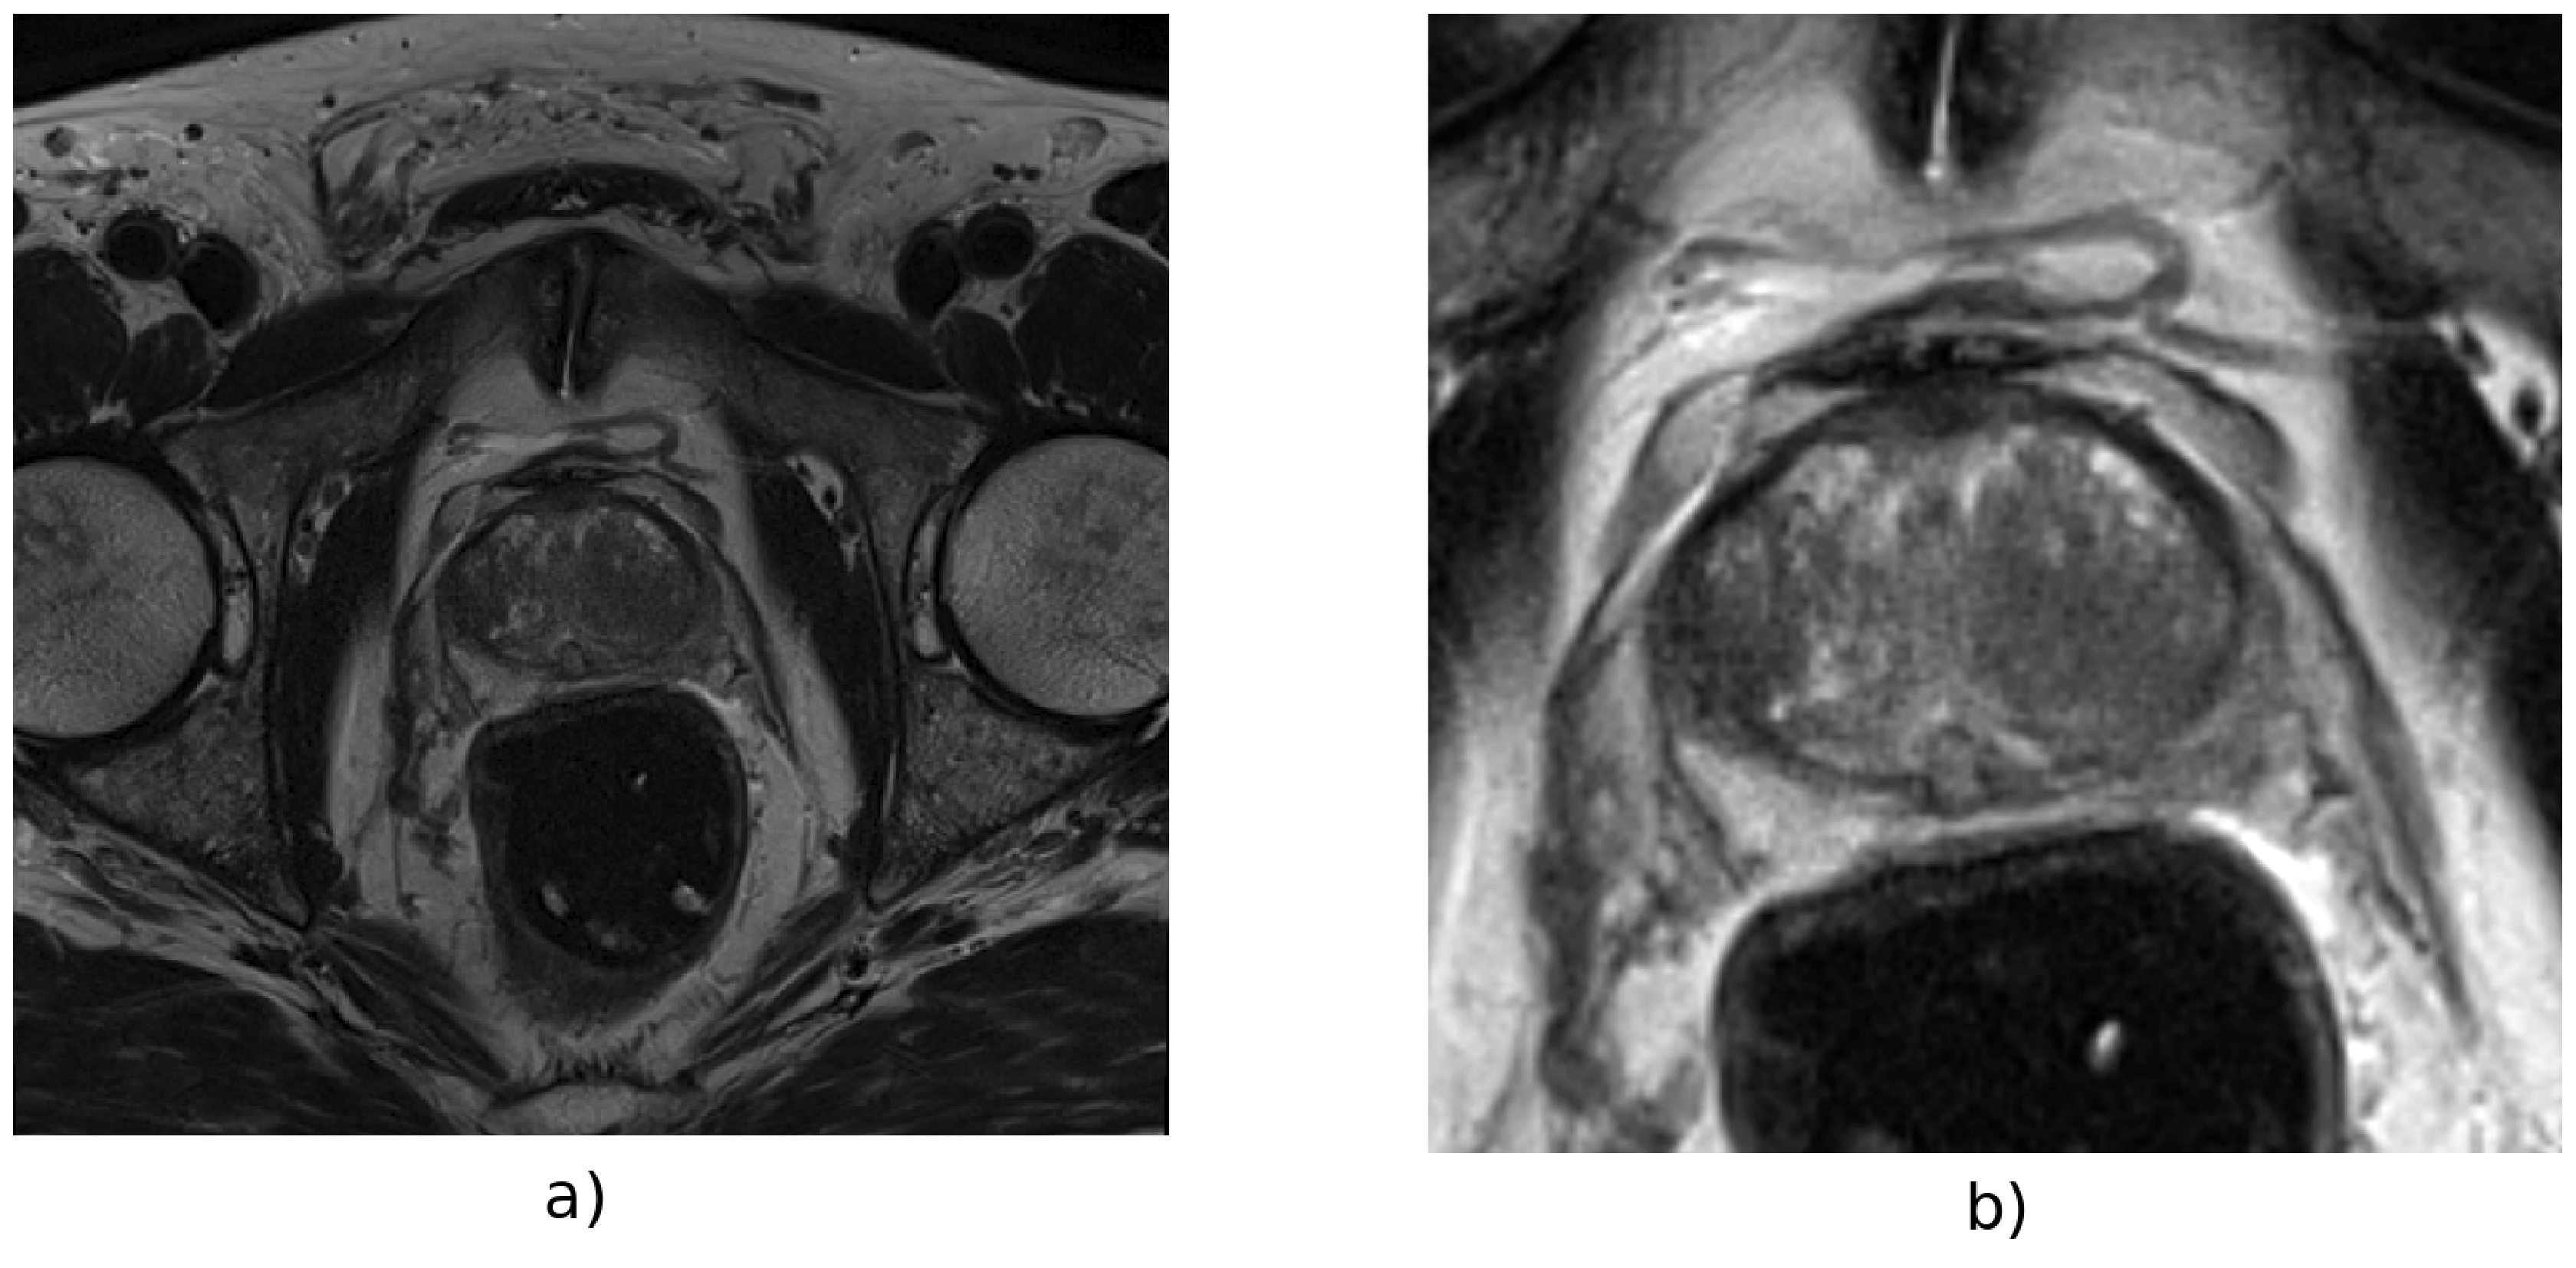
\includegraphics[totalheight=.25\textheight]{figures/Figure1.eps}
%    \caption{The MRIs are preprocessed with bias correction, normalization, resampling, and cropped to a ROI to reduce the variability of sizes and intensities between magnets. In this example, \textbf{a)} is the original image and \textbf{b)} is the image after being processed.} 
%    \label{fig_1}
%\end{figure}

Manual contours made by the experts were carried on the original MRI resolutions and not on the higher resolution version; therefore, the necessity for interpolating them.  The proposed interpolation is performed in two dimensions and is computed independently between every two consecutive horizontal slices. First, optical flow is obtained between the two contours using the Farneback method \cite{optflow}. Then, the contours are interpolated linearly following the direction of the optical flow. Figure \ref{fig:fig_2} shows an example of the optical flow obtained between two horizontal slices and the resulting interpolated contour using this method. 

%\begin{figure}[h]
%    \centering
%    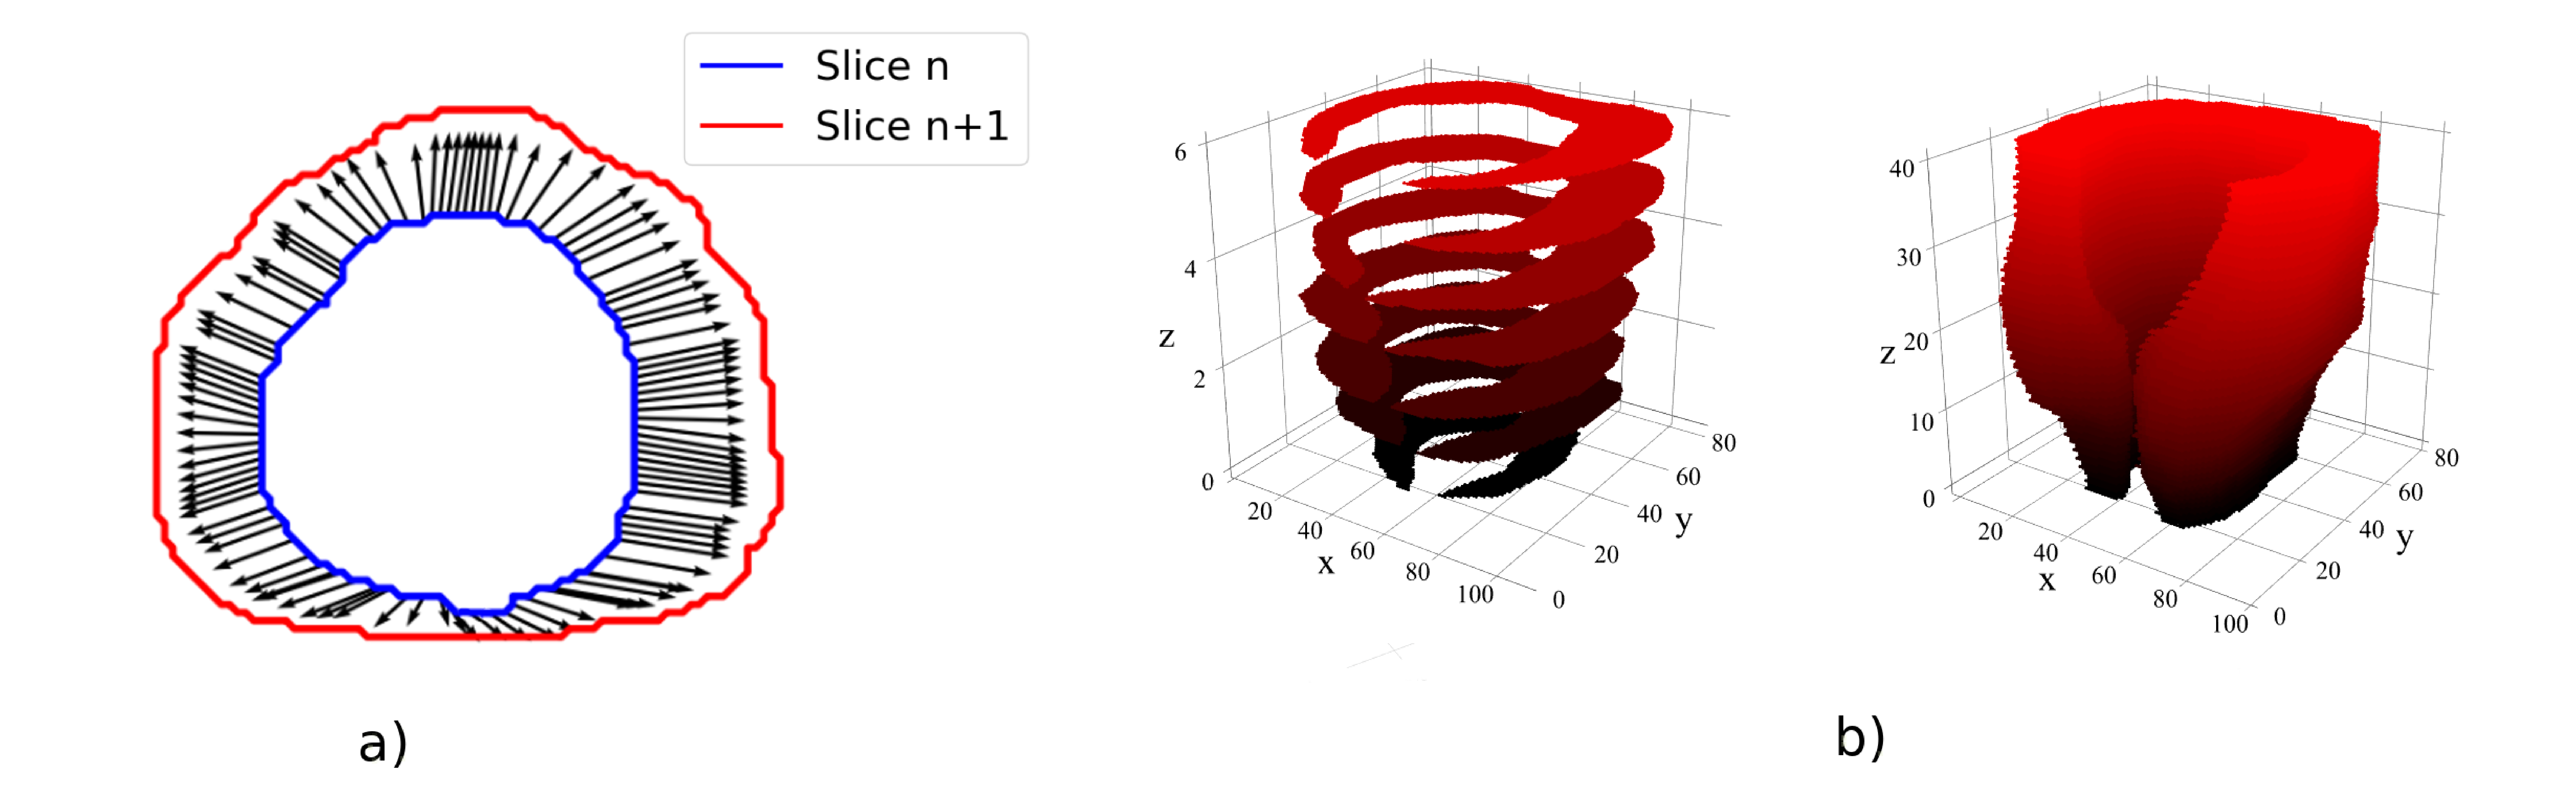
\includegraphics[totalheight=.21\textheight]{figures/Figure2.eps}
%    \caption{Example of the proposed algorithm to increase the resolution of prostate and PZ contours. In \textbf{a)}, an example of the optical flow obtained between two prostate contours from adjacent horizontal planes. In \textbf{b)} on the left, original contours with 17 slices. On the right, interpolated contours with 68 slices.}
%    \label{fig:fig_2}
%\end{figure}

